
\documentclass[a4paper,12pt]{article}
\usepackage[utf8]{inputenc}
\usepackage[T1]{fontenc}
\usepackage{graphicx}
\usepackage{caption}
\title{Esercizi dalle pagine 29, 31, 34 e 36}
\author{}
\date{}

\begin{document}
\maketitle

\section*{Esercizio pagina 29}
\begin{enumerate}
  \item \textbf{Aprire un secondo terminale e rilanciare il server. Funziona? Perché?}\\
    \emph{Risposta:} No, non funziona perché il socket è già occupato dall'altro processo.
    \begin{figure}[h]
      \centering
      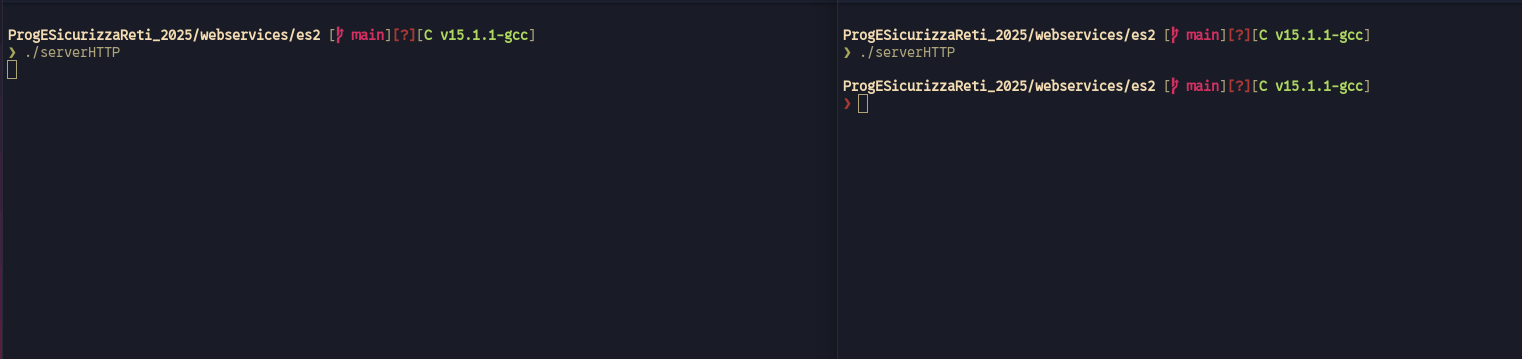
\includegraphics[width=0.7\linewidth]{due_server.png}
      \caption{Tentativo di avviare due istanze del server}
    \end{figure}

  \item \textbf{Aprire il browser e impostare la URL \texttt{http://127.0.0.1:8000/}. Cosa si vede sul browser e sul terminale?}\\
    \emph{Risposta:} Sul browser viene mostrata la pagina di prova, mentre nel terminale compare il log della richiesta.
    \begin{figure}[h]
      \centering
      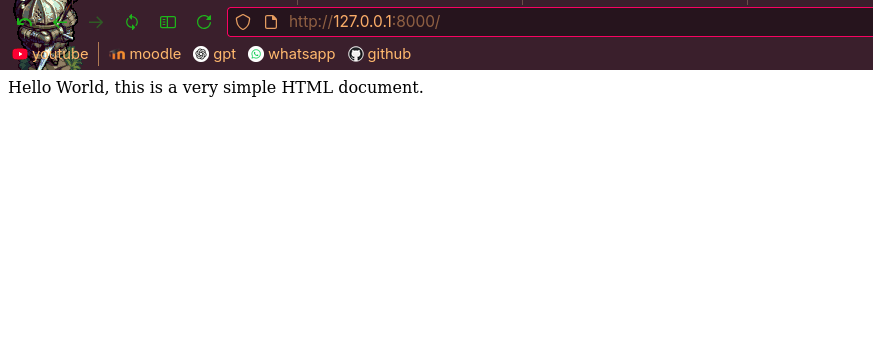
\includegraphics[width=0.45\linewidth]{browser1.png}
      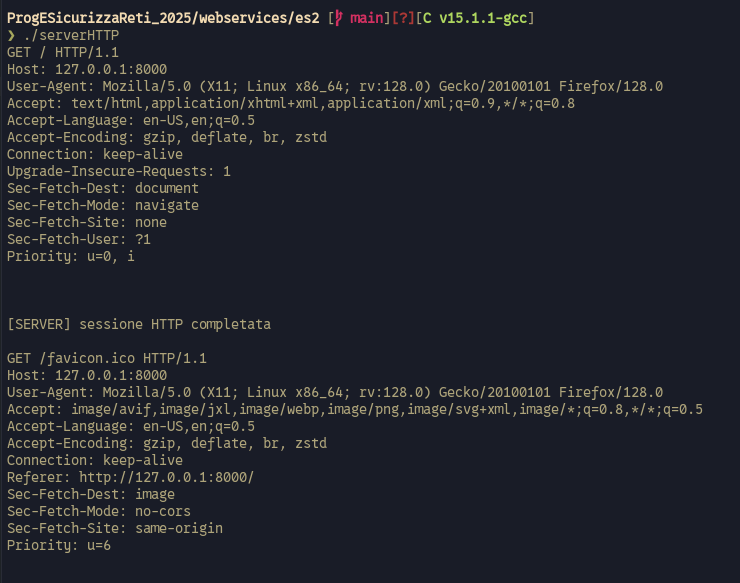
\includegraphics[width=0.45\linewidth]{terminale1.png}
      \caption{Visualizzazione di \texttt{127.0.0.1:8000} sul browser (sinistra) e sul terminale (destra)}
    \end{figure}

  \item \textbf{Impostare la URL \texttt{http://localhost:8000/}. Cosa cambia?}\\
    \emph{Risposta:} Cambia solo il valore dell'header \texttt{Host} nella richiesta HTTP, che diventa \texttt{localhost}.
    \begin{figure}[h]
      \centering
      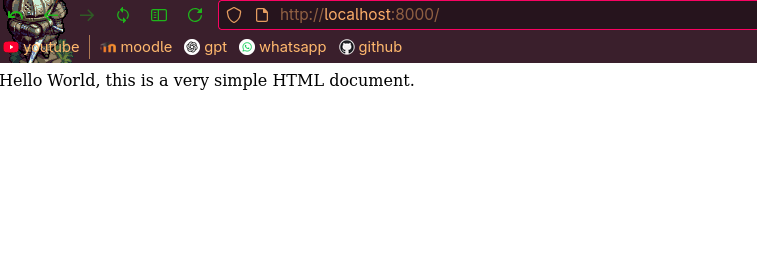
\includegraphics[width=0.45\linewidth]{browser2.png}
      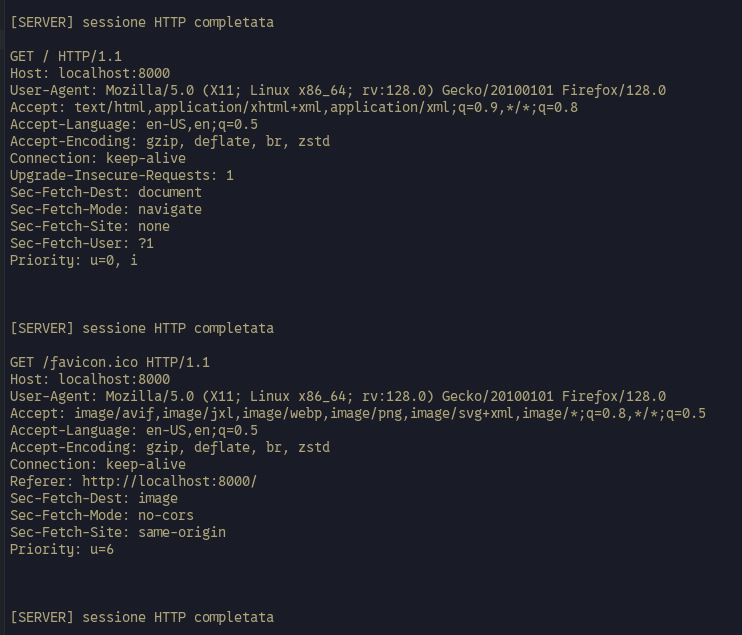
\includegraphics[width=0.45\linewidth]{terminale2.png}
      \caption{Visualizzazione di \texttt{localhost:8000} sul browser (sinistra) e sul terminale (destra)}
    \end{figure}
\end{enumerate}

\section*{Esercizio pagina 31}
\begin{enumerate}
  \item \textbf{Eseguire il server web e aprire \texttt{form-get.html}. Cosa si vede?}\\
    \emph{Risposta:} Viene visualizzato sempre ``Hello World, this is a very simple HTML document.'', cambia solo la pagina richiesta (\texttt{/form-get.html}).
    \begin{figure}[h]
      \centering
      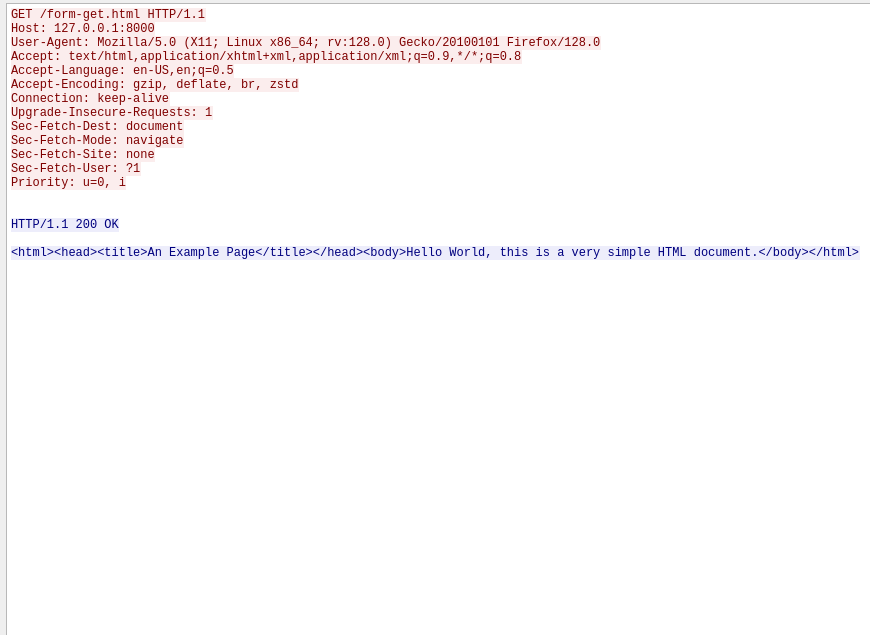
\includegraphics[width=0.7\linewidth]{form-get.png}
      \caption{Esecuzione con \texttt{form-get.html}}
    \end{figure}
\end{enumerate}

\section*{Esercizio pagina 34}
\begin{enumerate}
  \item \textbf{Eseguire il server web e aprire \texttt{form-post.html}. Cosa si vede?}\\
    \emph{Risposta:} Uguale a prima, viene mostrata la pagina di prova, cambia solo l'URL (\texttt{/form-post.html}).
    \begin{figure}[h]
      \centering
      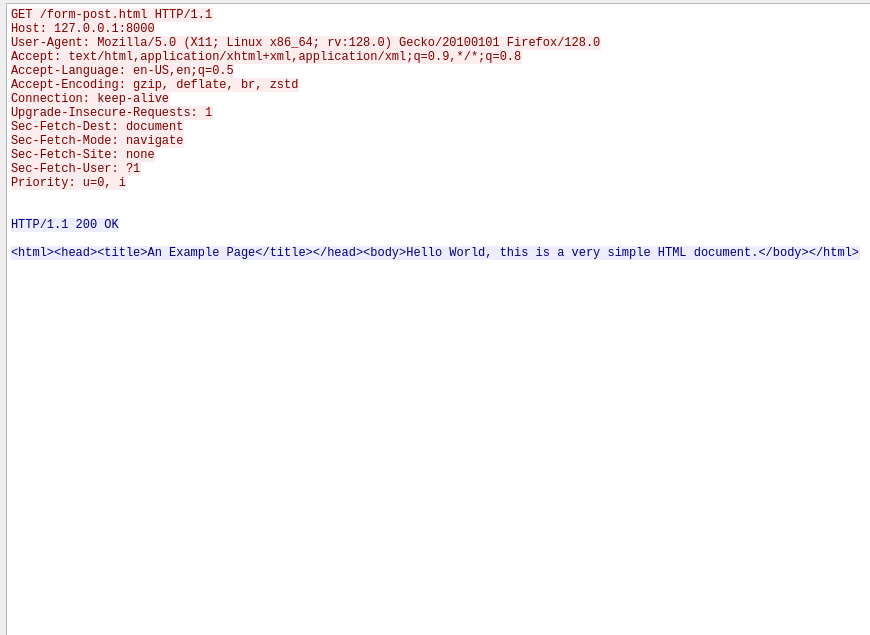
\includegraphics[width=0.7\linewidth]{form-post.png}
      \caption{Esecuzione con \texttt{form-post.html}}
    \end{figure}
\end{enumerate}

\section*{Esercizio pagina 36}
\begin{enumerate}
  \item \textbf{Modificare \texttt{serverHTTP.c} per restituire le pagine richieste (\texttt{form-get.html}, \texttt{form-post.html}). Cosa succede?}\\
    \emph{Risposta:} Le pagine corrispondenti vengono effettivamente restituite in base al path richiesto.
    \begin{figure}[h]
      \centering
      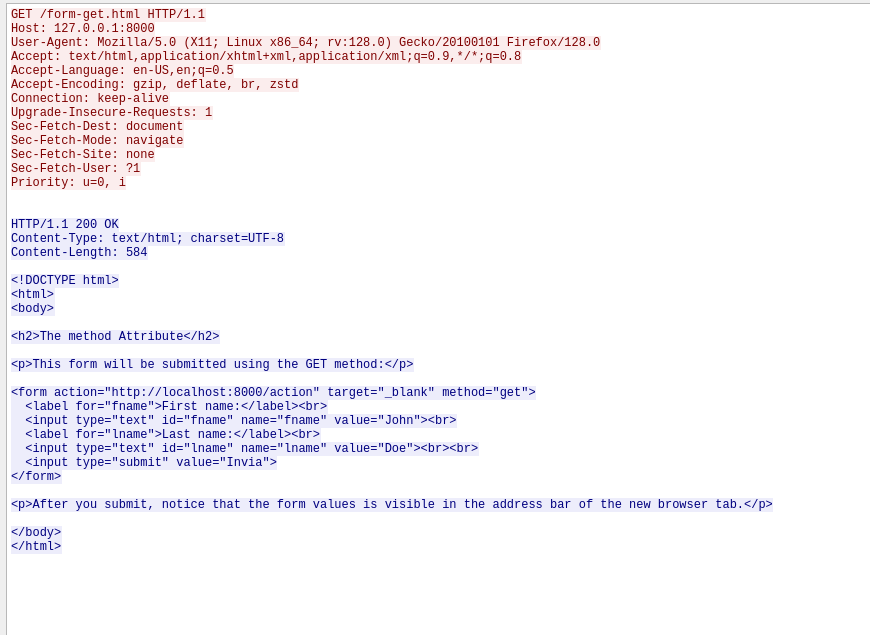
\includegraphics[width=0.7\linewidth]{form-get_corretto.png}
      \caption{Risultato dopo la modifica del server}
    \end{figure}
\end{enumerate}

\end{document}
